\subsection{A bounded test of explicit endpoint search}
Updating energy labels does not directly follow an energy gradient. We
therefore run a separate discrete search pilot to test the value of feedback
from an actual MLIP evaluation. It begins only after the core experiment is
complete and after all causal-control proposal identities have been reserved.

At each of the three lithium counts, LOW and HIGH searches begin from 16
unprotected H0 TRAIN masks per seed. Greedy and energy-blind walks share those
starts. At each of four steps, each trajectory proposes eight edits, each
exchanging one occupied and one vacant Li site. This is one swap in occupancy
space, not a physical diffusion trajectory. The greedy walk chooses the
lowest- or highest-energy eligible neighbor according to UMA; ties use a
declared canonical-mask order. The blind walk's chosen neighbor and its
eligibility-only fallback are written before any new energy is evaluated.
Both walks query the full eligible candidate union. Their first-step raw
proposals and query unions are checked to be exactly identical.

A uniform fixed-count sampler receives the same attempt/query caps, without
a claim of identical edit semantics. Each arm has at most 128 attempts and
new queries per count/direction/step, or 512 over four steps. Known,
protected, and repeated orbits remain excluded without top-ups. Actual
selected query counts are retained, and shared geometry--teacher evaluations
are physically performed only once.

\begin{table}[htbp]
\centering\small
\caption{Best observed UMA energy gain relative to the same starting-pool
best, in meV/atom, mean $\pm$ sample SD over three paired seeds. Positive
LOW gain means lower energy; positive HIGH gain means higher energy.
The reference is the best of the common 16 starts, not the minimum or
maximum of the entire H0 dataset.}
\begin{tabular}{llrrr}\toprule
Li count & Direction & Greedy & Blind walk & Uniform\\\midrule
12 & LOW  & $2.17\pm0.67$ & $1.38\pm0.97$ & $1.33\pm0.89$\\
24 & LOW  & $2.06\pm1.02$ & $1.05\pm0.65$ & $1.20\pm1.63$\\
36 & LOW  & $2.82\pm0.65$ & $1.21\pm0.29$ & $1.19\pm0.24$\\
12 & HIGH & $8.26\pm3.38$ & $3.70\pm0.14$ & $2.04\pm2.15$\\
24 & HIGH & $5.29\pm2.87$ & $4.61\pm3.34$ & $1.75\pm2.42$\\
36 & HIGH & $5.45\pm2.25$ & $1.93\pm1.31$ & $1.31\pm1.72$\\
\bottomrule\end{tabular}
\end{table}

Within this bounded budget, energy feedback improves the mean observed LOW
endpoint relative to both declared controls at all three counts. MACE audits
the same queried structures independently and shows the same qualitative
LOW advantage: greedy gains are 2.33, 2.16, and 2.46 meV/atom at counts
12, 24, and 36. MACE does not choose the next states. The HIGH advantage is
less uniform across counts and replicates, particularly at count 24.
These small paired experiments do not establish a universal ordering of
the methods.

\begin{figure}[htbp]
\centering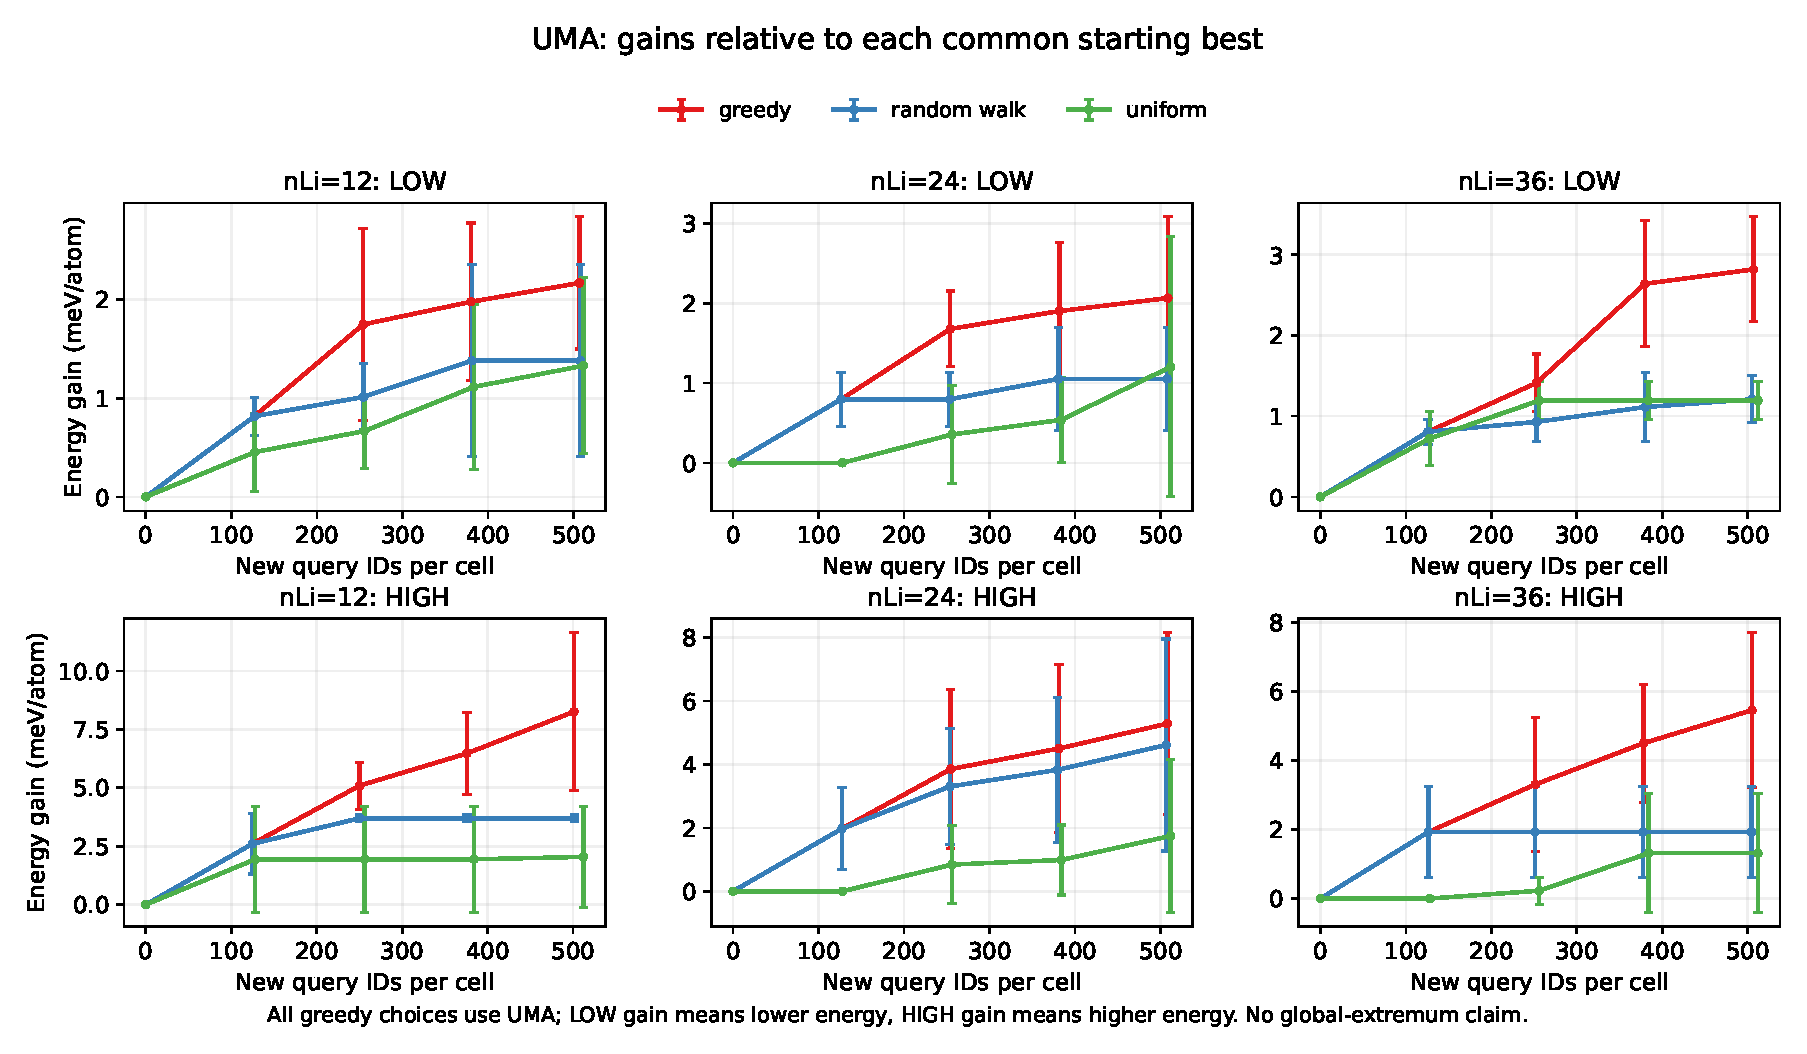
\includegraphics[width=\linewidth]{frontier_uma_best_gain.pdf}
\caption{Observed endpoint gains versus actual newly scored cell-query IDs.
Greedy and blind walks have identical first-step queries and fixed one-swap,
eight-neighbor budgets. Uniform has equal caps but different proposal
semantics. Best-so-far includes every evaluated neighbor and is monotone
by construction. Selected current paths are logged separately and may leave
an earlier best; the retained best and current state are different objects.
Error bars show three-seed sample SD.}
\end{figure}

No neural edit model is trained in this pilot. It separates label
redistribution from explicit oracle-guided search and cannot be treated as
a matched-edit comparison with the CVAE decoder. The new evaluations cover
49,570 geometry--teacher pairs, plus 574 separate rescoring evaluations of
287 distinct TRAIN seed masks. The pilot completes in 30.88 minutes within
its declared cap, with all raw checks passing.

Exact orbit filtering applies to all arms. Current-state uniqueness is
partly imposed by that filter, so it is not evidence of unrestricted
diversity. The saved diversity diagnostic instead uses the minimum Hamming
distance over parent symmetries, divided by two: the number of Li/vacancy
swaps separating two masks. The comparison uses the 16 current walk states
or the first 16 eligible uniform proposals without energy selection.
All coordinates remain unrelaxed. The results concern observed surrogate
endpoints, not global extrema, configurational entropy, equilibrium phase
stability, or DFT validation.
